% !TEX root = ../Dissertation.tex

\section{Results}
\label{sec:results}

This section presents the empirical results of the experiments detailed in Section 5.1. The performance of our proposed Transformer-PPO model is objectively compared against all baseline solvers using the metrics of solution quality (MRE) and computational efficiency (inference time).

\subsection{Quantitative Performance Summary}
The primary quantitative results are summarized in Table~\ref{tab:main_results}. This table presents the Mean Relative Error (MRE) and average inference time for each solver across four representative problem sizes, from small ($n=50$) to large ($n=200$). The data clearly illustrates the trade-offs between solution quality, computational speed, and scalability for each approach. Our proposed PPO model consistently achieves a low MRE on large-scale instances while maintaining a practical inference time.

\begin{table}[htbp]
    \centering
    \caption{Performance Comparison of Solvers on the Generalization Test Set}
    \label{tab:main_results}
    
    \setlength{\tabcolsep}{4pt} 
    
    \small
    \begin{tabular}{@{}lcccccccc@{}}
        \toprule
        
        & \multicolumn{4}{c}{\textbf{MRE (\%)}} & \multicolumn{4}{c}{\textbf{Time (ms)}} \\
        
        \cmidrule(lr){2-5} \cmidrule(lr){6-9}
        \textbf{Model} & \textbf{n=50} & \textbf{n=100} & \textbf{n=150} & \textbf{n=200} & \textbf{n=50} & \textbf{n=100} & \textbf{n=150} & \textbf{n=200} \\
        \midrule
        Gurobi & 0.00 & 0.00 & 0.00 & 0.00 & 0.58 & 2.10 & 4.16 & 4.22 \\
        MLP/DNN & 42.16 & 83.13 & 94.62 & 100.00 & 0.81 & 0.84 & 0.65 & 0.70 \\
        Prt-Net & 99.16 & 99.30 & 99.41 & 100.00 & 13.01 & 12.50 & 13.14 & 13.00 \\
        \textbf{PPO (Ours)} & \textbf{13.79} & \textbf{28.11} & \textbf{29.89} & \textbf{29.53} & 198.54 & 406.40 & 610.87 & 819.57 \\
        \bottomrule
    \end{tabular}

    \begin{minipage}{0.95\textwidth}
        \small
        \vspace{2pt}
        \textbf{Note:} MRE is calculated against Gurobi's optimal solutions; lower is better.
    \end{minipage}
\end{table}

% In your LaTeX preamble, make sure you have: \usepackage{subcaption}

\subsection{Visual Analysis}
To better visualize the performance trends as the problem size increases, the key results for solution quality and computational efficiency are presented graphically in Figure~\ref{fig:visual_results}.

\begin{figure}[htbp]
    \centering

    % --- First Subfigure (MRE Plot) ---
    \begin{subfigure}{\textwidth}
        \centering
        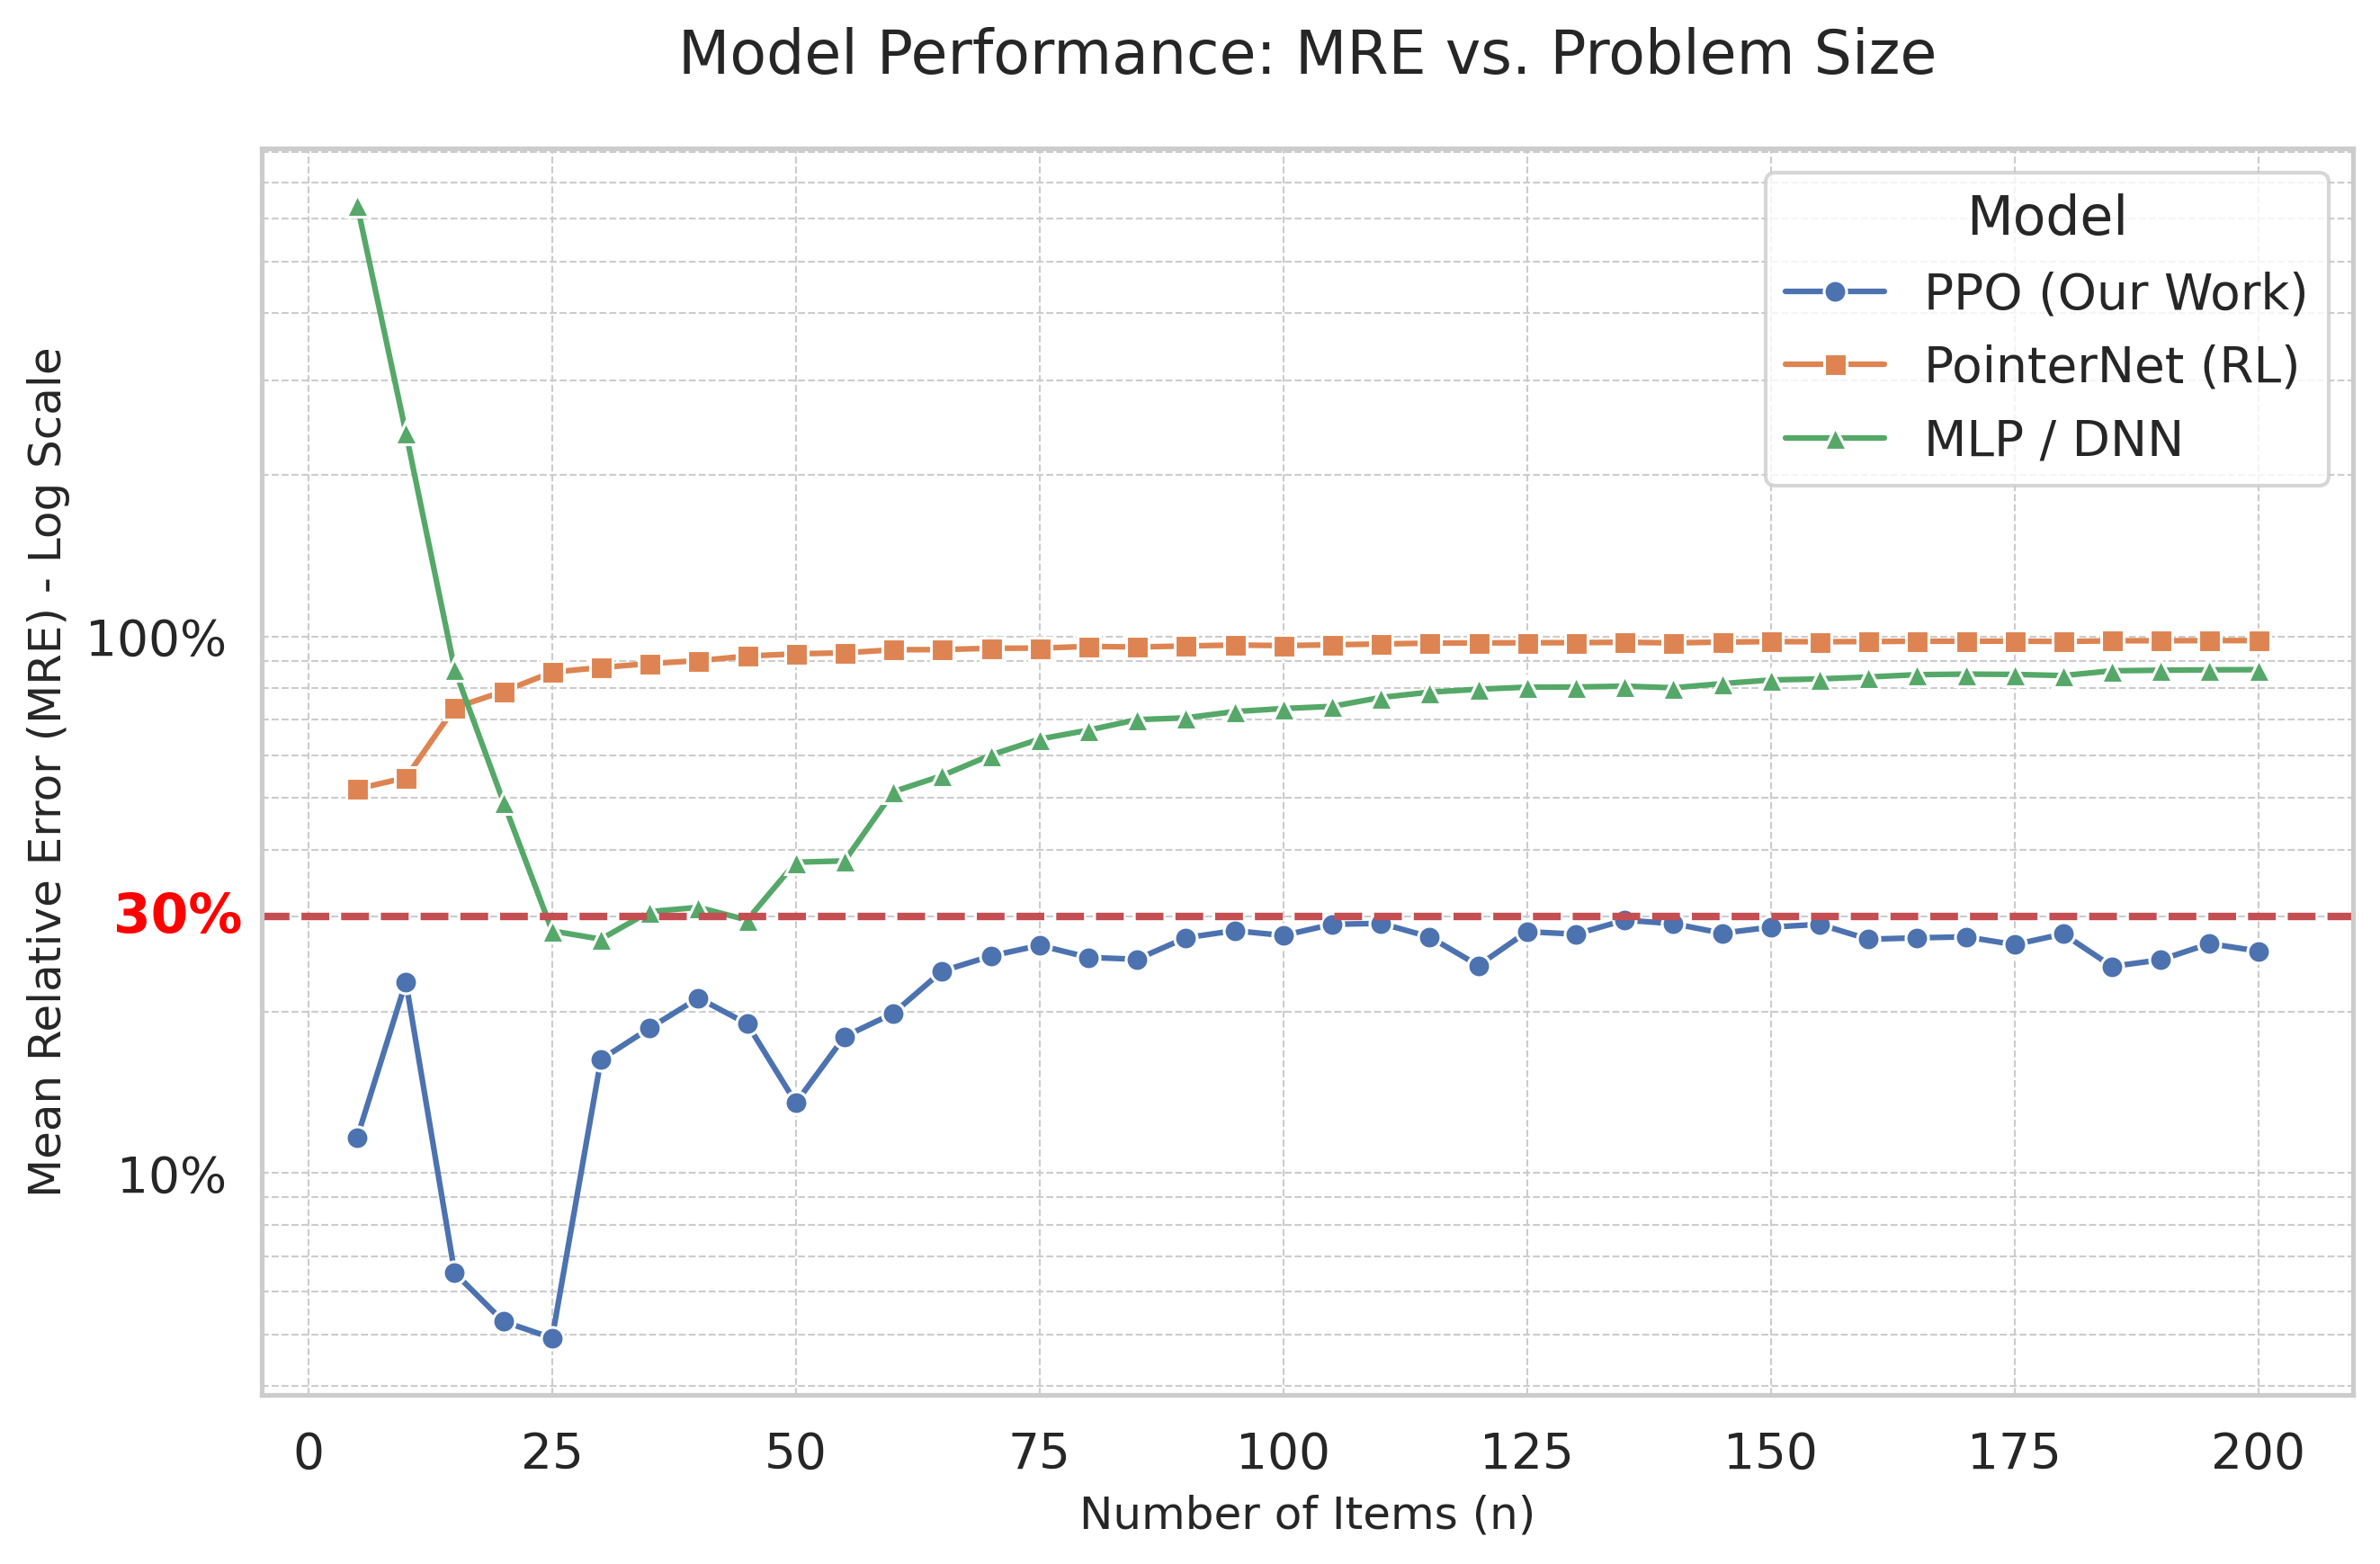
\includegraphics[width=0.9\textwidth]{figures/mre_vs_problem_size_styled.png}
        \caption{Model Performance: MRE vs. Problem Size.}
        \label{fig:mre_vs_size}
    \end{subfigure}

    \vspace{1em} % Adds a vertical space between the two plots

    % --- Second Subfigure (Time Plot) ---
    \begin{subfigure}{\textwidth}
        \centering
        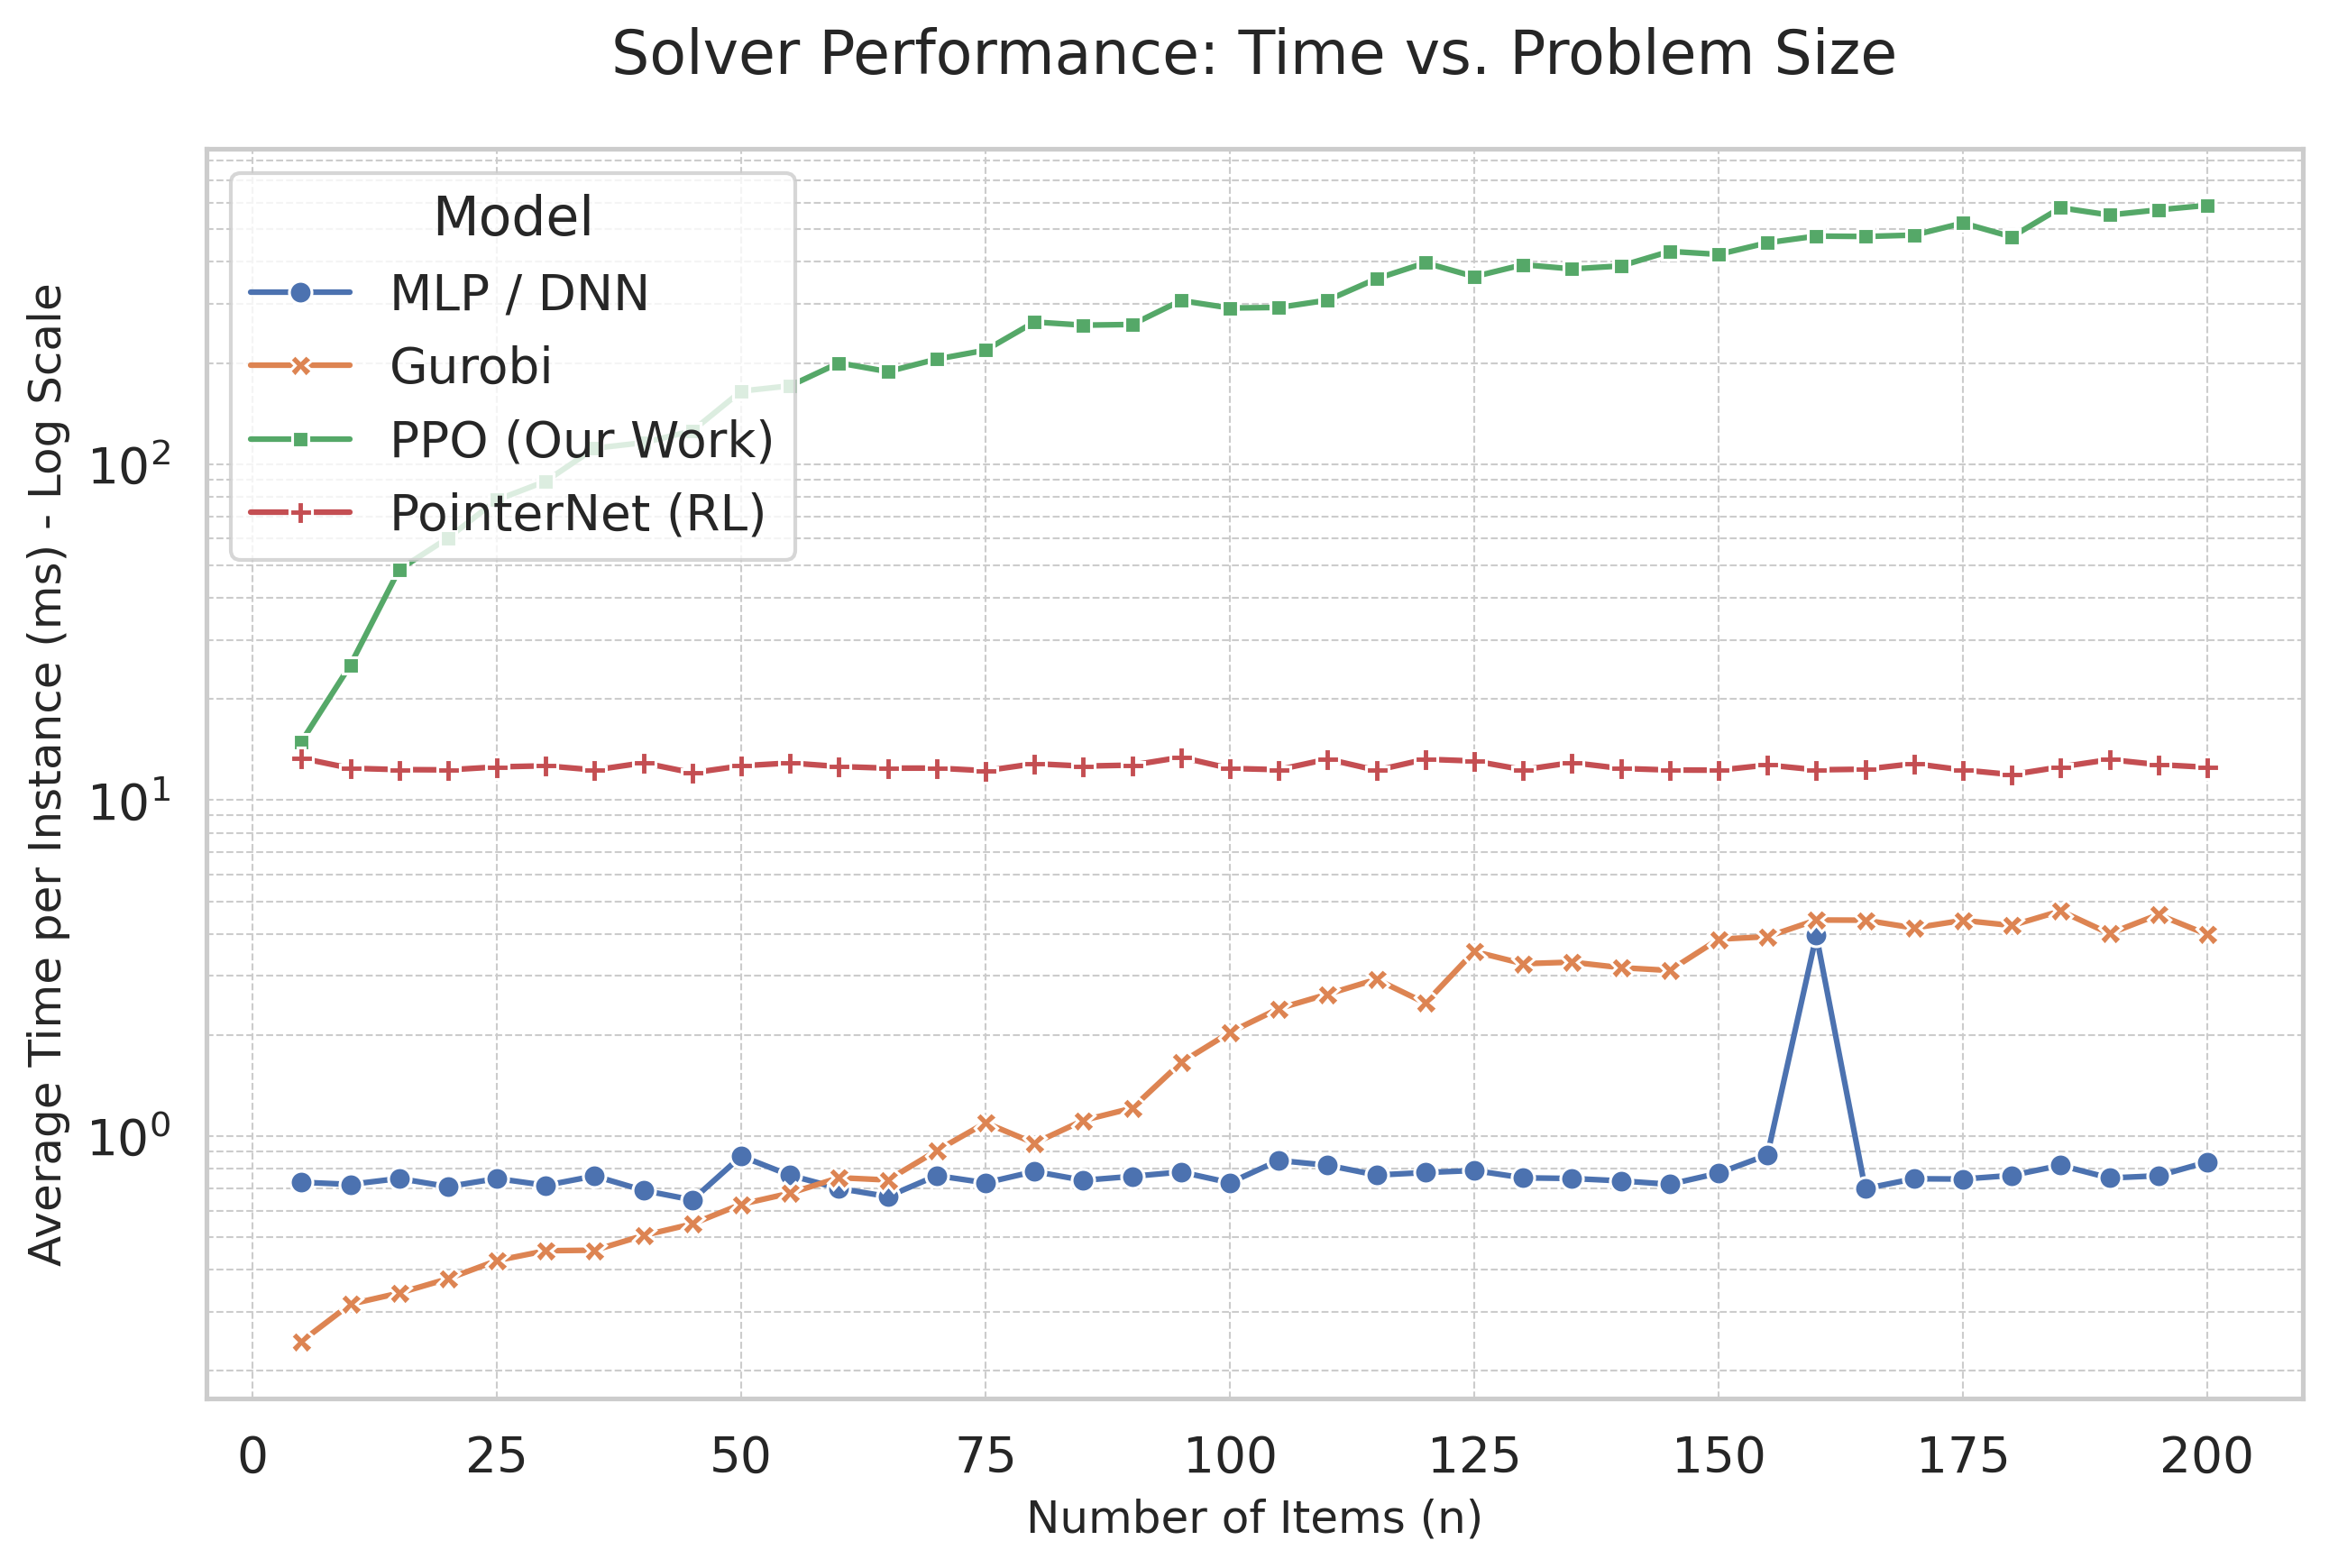
\includegraphics[width=0.9\textwidth]{figures/evaluation_times_vs_n_styled.png}
        \caption{Solver Performance: Time vs. Problem Size (Log Scale).}
        \label{fig:time_vs_size}
    \end{subfigure}
    
    % --- Main Caption for the entire figure ---
    \caption{Visual analysis of solver performance. (a) Our PPO model demonstrates effective generalization, maintaining a stable, low error rate on large instances. (b) The neural network models are significantly faster than the optimal Gurobi solver on larger instances.}
    \label{fig:visual_results}
\end{figure}

The plot of Mean Relative Error (Figure~\ref{fig:mre_vs_size}) clearly demonstrates the strong generalization capability of our proposed PPO model. While its error is initially higher on very small instances, it quickly stabilizes below the 30\% threshold as the problem size grows, indicating that it has learned a robust, scalable policy. In contrast, the MLP/DNN model's performance degrades rapidly, and the REINFORCE-trained Pointer Network fails to converge to a meaningful policy, maintaining a near-100\% error rate.

Figure~\ref{fig:time_vs_size} illustrates the average inference time per instance for each solver. This log-scale plot highlights the computational efficiency of the different approaches. The neural methods (MLP, Pointer Network, and PPO) exhibit favorable scaling, with their inference times growing much slower than the Gurobi solver. Although our PPO model is the most computationally intensive of the neural approaches due to its Transformer architecture, it remains orders of magnitude faster than Gurobi on large instances, confirming its practicality for applications requiring rapid decision-making.
